\documentclass[conference]{IEEEtran}
\IEEEoverridecommandlockouts
\usepackage{cite}
\usepackage{amsmath,amssymb,amsfonts}
\usepackage{algorithmic}
\usepackage{graphicx}
\usepackage{textcomp}
\usepackage{xcolor}
\usepackage{booktabs}
\usepackage{bm}
\def\BibTeX{{\rm B\kern-.05em{\sc i\kern-.025em b}\kern-.08em
    T\kern-.1667em\lower.7ex\hbox{E}\kern-.125emX}}
\begin{document}

\title{FQCNN: A Fully Quantum-Native Convolutional\\ Neural Network with Coherent Unitary Pooling}

\author{\IEEEauthorblockN{Aasa Singh Bhui}
\IEEEauthorblockA{\textit{School of Computer Science} \\
\textit{and Engineering} \\
\textit{Vellore Institute of Technology}\\
Vellore, India \\
Fourth-year B.Tech, Computer Science \\
aasasingh2005@gmail.com}
\and
\IEEEauthorblockN{Prithvi Raghu}
\IEEEauthorblockA{\textit{School of Computer Science} \\
\textit{and Engineering} \\
\textit{Vellore Institute of Technology}\\
Vellore, India \\
Third-year B.Tech, Computer Science \\
prithviraghu080706@gmail.com}
\and
\IEEEauthorblockN{Rohan Jain}
\IEEEauthorblockA{\textit{Director of DevOps \& Delivery} \\
\textit{AstraZeneca}\\
Gaithersburg, Maryland, USA \\
rohan.jain7@gmail.com}
}

\maketitle

\begin{abstract}
Building a quantum convolutional neural network that stays coherent throughout the circuit remains difficult. Near-term devices are limited in depth and noise tolerance, so most quantum machine learning models either combine classical and quantum processing or rely on measurement-based pooling, both of which collapse the quantum state and constrain the architecture. We propose a model that performs data encoding, local convolution, pooling, and classification using only unitary quantum operations. It uses amplitude encoding for compact representation, a parameter-shared SU(2) quantum convolutional kernel for local feature extraction, and a mid-circuit measurement-free pooling layer, which transfers information through parameterized controlled unitary operations instead of destructive projective measurements. The circuit is kept shallow and parameter-efficient to suit NISQ devices, and the pooling layer architecture ensures that physical reset overheads are bypassed while allowing execution on standard feed-forward quantum backends. In our experiments the model achieves approx 98\% test accuracy while remaining coherent across all layers. The results suggest that fully unitary hierarchical quantum models can perform competitively without intermediate measurements, which is useful for scaling quantum machine learning.
\end{abstract}

\begin{IEEEkeywords}
Quantum convolutional neural networks, variational quantum circuits, quantum machine learning, amplitude encoding, unitary pooling, NISQ computing, coherent quantum architectures.
\end{IEEEkeywords}

\section{Introduction}
Quantum machine learning has become an active research area that studies how quantum computing can be applied to data-driven, learning-based tasks. One recurring interest is how to bring useful inductive biases, such as locality, parameter sharing, and hierarchical feature extraction, into the quantum setting. Among classical models, the convolutional neural network has been especially successful because it exploits spatial structure in data, which motivated quantum convolutional neural networks (QCNNs) that aim to carry the principles of classical CNNs into quantum circuits~\cite{ref45}.

Several approaches have extended convolutional ideas to the quantum domain through structured variational circuits, usually referred to as QCNNs. These models tend to rely on hierarchical constructions that apply local quantum operations followed by dimensionality reduction~\cite{ref46}. Recent work has explored a range of architectural variants, including hardware-aware QCNN designs that minimise circuit depth and qubit requirements, along with flexible convolutional schemes that adjust stride or windowing to improve scalability on near-term noisy intermediate-scale quantum (NISQ) devices~\cite{ref2,ref6,ref7}. To gauge practical performance, benchmarking studies have analysed QCNN behaviour across classification and compression tasks, drawing out the trade-offs between expressibility, parameter count, and trainability~\cite{ref8}. In many existing implementations, pooling is realised through mid-circuit measurements or classical post-processing, which disrupts the established quantum coherence and limits the model's ability to preserve quantum correlations across layers~\cite{ref4}. Other studies have looked at trainability challenges in QCNN architectures, including the barren plateau phenomenon, which has motivated architectural constraints and mitigation strategies aimed at stabilising the learning dynamics~\cite{ref11}.

Substantial as these advances are, several limitations still hinder effective deployment on near-term hardware. Reliance on measurement-based pooling or hybrid classical--quantum architectures introduces an irreversible loss of quantum information, which prevents coherent feature hierarchies from forming across convolutional layers. Many proposed architectures also employ globally entangling circuits or deep variational blocks, and these intensify noise accumulation and gradient instability as the system grows. Hardware-aware designs reduce the resource requirements, but often at the cost of expressivity or coherence preservation. A gap therefore remains: we still lack QCNN architectures that hold full quantum coherence across the whole learning pipeline while staying shallow, parameter-efficient, and trainable under realistic noise and connectivity constraints.

These limitations matter most on NISQ devices, where noise, short coherence times, and restricted qubit connectivity place tight constraints on circuit design. Architectures that depend on deep variational blocks or frequent mid-circuit measurements are particularly exposed to decoherence and error accumulation, which leads to unstable training and poor generalisation. Losing coherence between convolutional layers also undermines the hierarchical feature extraction that motivates convolutional architectures in the first place. As NISQ hardware scales incrementally rather than exponentially, there is growing value in models that emphasise shallow depth, locality-preserving operations, and parameter efficiency while keeping information flowing coherently through the circuit.

In this work we address these challenges by introducing a fully quantum-native neural network (FQCNN) architecture designed to preserve coherence across every stage of the learning pipeline. The model performs data encoding, convolution, pooling, and classification entirely through unitary operations, removing the need for intermediate measurement or classical post-processing. Local quantum convolution is implemented with a shared 2$\times$2 kernel acting on spatially adjacent qubits, which enforces parameter sharing and a translational inductive bias while keeping circuit depth low. Dimensionality reduction is achieved through a coherent pooling mechanism that uses unitaries to compress information without collapsing the state or breaking the established entanglement.

Beyond its architectural advantages, the model also performs strongly in practice, reaching approx 98\% test accuracy on a binary classification task while maintaining quantum coherence throughout the computation. This suggests the architecture is physically consistent with quantum hardware constraints.

The main contributions of this work are as follows:
\begin{enumerate}
\item We propose a fully quantum-native convolutional neural network that maintains coherence across encoding, convolution, pooling, and classification, with no intermediate disruption or classical post-processing.
\item We introduce a local, parameter-shared quantum convolutional kernel that enforces a spatial inductive bias while staying shallow and hardware-efficient.
\item We develop a coherent unitary pooling mechanism that performs dimensionality reduction through quantum operations alone.
\item We demonstrate the architecture empirically, reaching approx 98\% classification accuracy under realistic training conditions.
\end{enumerate}

The rest of the paper is organised as follows. Section II reviews related work on quantum convolutional and variational quantum models. Section III describes the proposed FQCNN architecture and its mathematical formulation. Section IV covers the training dynamics and optimisation strategy. Section V reports the experimental results and analysis. Section VI details the novelty and technical differentiation, and Section VII concludes with limitations and future directions.

\begin{figure*}[!t]
\centering
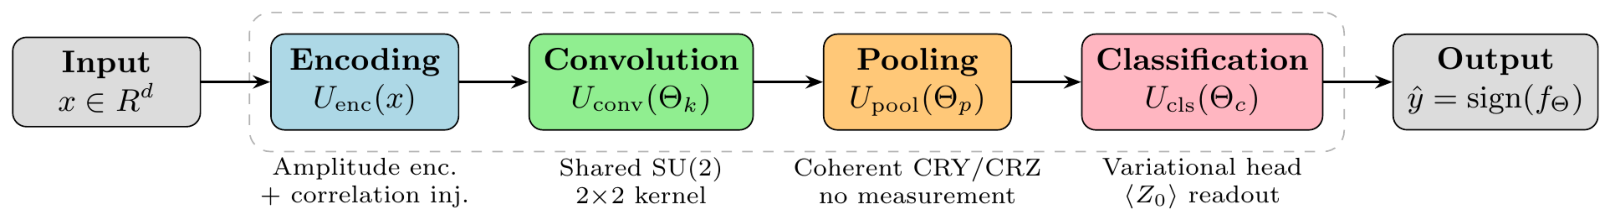
\includegraphics[width=\textwidth]{figs_final/fig1.png}
\caption{Overall FQCNN architecture. The pipeline runs Input $\rightarrow$ Encoding $\rightarrow$ Convolution $\rightarrow$ Pooling $\rightarrow$ Classification $\rightarrow$ Output. Every stage operates through unitary quantum operations, with no intermediate measurements.}
\label{fig:arch}
\end{figure*}

\section{Related Work}
\subsection{Quantum Convolutional Neural Networks}
Quantum convolutional neural networks extend classical convolutional networks into the quantum domain by combining local unitary operations with hierarchical dimensionality reduction. Early formulations used structured variational circuits inspired by renormalisation techniques~\cite{ref37}, while more recent work adopts hardware-aware adaptations that cut circuit depth and qubit requirements to suit near-term devices~\cite{ref2,ref6,ref7}. Convolutional mechanisms that emphasise flexibility, including modified stride strategies and pointwise approaches, have been proposed to improve scalability and adaptability under connectivity constraints~\cite{ref6,ref36}. Benchmarking studies evaluate QCNN performance across classification and compression tasks, highlighting trade-offs between parameter efficiency, expressibility, and noise robustness~\cite{ref8}. Despite this progress, many variants still use measurement-based pooling or hybrid components that disrupt established coherence and limit fully unitary hierarchical representations~\cite{ref4}.

\subsection{Variational Quantum Classifiers and Trainability}
The broader framework of variational quantum circuits (VQCs) underlies most quantum machine learning models~\cite{ref40}. Optimisation typically relies on gradient-based methods such as the parameter-shift rule and stochastic descent variants~\cite{ref13,ref21,ref41}. Increasing circuit depth and expressibility does not always help; it can produce barren plateaus, where gradient magnitudes vanish exponentially with system size~\cite{ref14,ref17,ref19,ref38}. Several strategies soften these effects, including structured ansatz design, reduced-domain parameter initialisation, and architecture-aware optimisation~\cite{ref11,ref18,ref47}. More recent developments, such as stochastic quantum Hamiltonian descent and Bayesian optimisation, explore alternative training paradigms aimed at stabilising convergence in noisy settings~\cite{ref10,ref15}. Together, these findings show that architectural constraints and locality are important for keeping scalable quantum models trainable.

\subsection{Quantum Autoencoders and Information Compression}
Dimensionality reduction in quantum models is often expressed through quantum autoencoder frameworks, which compress quantum states into lower-dimensional subspaces while preserving the relevant information~\cite{ref25,ref26}. Extensions have explored image classification and information compression through structured encoding--decoding circuits~\cite{ref3,ref23,ref29}. Autoencoders offer a principled route to quantum information compression, but they typically require extra circuit depth and can introduce optimisation difficulties under noise. By contrast, embedded pooling mechanisms that operate directly within QCNN architectures provide an alternative path to information reduction without separate encoding--decoding stages.

\subsection{Noise and Error Mitigation in Quantum Learning}
Noise remains the primary obstacle to deploying quantum machine learning models on near-term hardware. Comprehensive reviews of quantum error mitigation point to strategies such as zero-noise extrapolation, data-driven correction, and probabilistic error cancellation~\cite{ref22}. More recent approaches incorporate machine learning into the error mitigation pipeline, including neural-network-assisted correction and noise-agnostic data augmentation~\cite{ref16,ref20}. While these methods improve robustness at the hardware level, architectural strategies that reduce circuit depth and preserve locality offer a complementary path to noise resilience in quantum learning systems.

\section{Proposed FQCNN Architecture}
\subsection{Problem Formulation}
Consider a labelled dataset $\mathcal{D} = \{(x^{(k)}, y^{(k)})\}$ for $k = 1, \ldots, N$ in a supervised setting, where $x \in \mathbb{R}^d$ is the input feature vector, $x_i \in [-1, 1]$, $y \in \{-1, 1\}$, and $d$ is the number of features after preprocessing. To scale efficiently, we use amplitude encoding, which maps the input vector into a quantum state. We consider a register of $n = 10$ qubits all initialised in the ground state
\begin{equation}
|\psi_0\rangle = |0\rangle^{\otimes 10}.
\end{equation}
A two-dimensional input image $X \in \mathbb{R}^{28 \times 28}$ is flattened into a 784-dimensional vector $x$, which is zero-padded to 1024 and mapped to the $2^{10} = 1024$ state amplitudes using global amplitude encoding. The full model is a parameterised unitary circuit built from the following operations:
\begin{equation}
U(\Theta; x) = U_{\text{cls}}(\theta_c)\, U_{\text{pool}}(\theta_p)\, U_{\text{conv}}(\theta_k)\, U_{\text{enc}}(x),
\end{equation}
where $\Theta = \{\theta_c, \theta_p, \theta_k\}$. The scalar model output is defined as
\begin{equation}
f_\theta(x) = \langle\psi_0|U^\dagger(\Theta; x)\, Z_0\, U(\Theta; x)|\psi_0\rangle,
\end{equation}
and classification is performed via
\begin{equation}
\hat{y}(x) = \text{sign}\big(f_\theta(x)\big).
\end{equation}
All intermediate transformations are strictly unitary, with no mid-circuit measurements.

\subsection{Quantum Data Encoding}
This stage defines a structured quantum feature map that combines independent single-qubit embeddings with local, data-dependent entanglement. Unlike standard feature-map strategies~\cite{ref39,ref43}, we use amplitude encoding, which maps a normalised classical input vector into the amplitudes of the quantum state. This represents a $d$-dimensional input using only $\log_2(d)$ qubits, improving scalability while preserving global information. Prior to encoding, each input feature is min-max normalised to the bounded domain $[a, b] = [0, 1]$:
\begin{equation}
x_i' = \frac{x_i - x_{\min}}{x_{\max} - x_{\min}} \cdot (b - a) + a, \qquad [a, b] = [0, 1].
\end{equation}
The encoding factorises as
\begin{equation}
U_{\text{enc}}(x) = U_{\text{corr}}(x)\, U_{\text{loc}}(x).
\end{equation}

\subsubsection{Local quantum feature map}
For every qubit $i \in \{1, \ldots, N\}$, we define
\begin{equation}
U_i(x_i) = R_y\!\left(\tfrac{\pi}{2} x_i\right) R_z(\pi x_i)\, H.
\end{equation}
These act as a supplementary feature map layered on top of the amplitude encoding, adding local rotations and expressivity without increasing the qubit count~\cite{ref48}. The parameterised rotations are
\begin{equation}
R_z(\theta) = e^{-i\theta Z/2}, \qquad R_y(\theta) = e^{-i\theta Y/2},
\end{equation}
with the Hadamard gate
\begin{equation}
H = \frac{1}{\sqrt{2}}\begin{bmatrix} 1 & 1 \\ 1 & -1 \end{bmatrix}.
\end{equation}
The global embedding unitary is
\begin{equation}
U_{\text{loc}}(x) = \bigotimes_{i=1}^{N} U_i(x_i).
\end{equation}

\subsubsection{Local correlation injection}
Let the qubits be indexed linearly by $i \in \{1, \ldots, n\}$ along a one-dimensional register. We define the set of nearest-neighbour edges on a cyclic ring as
\begin{equation}
E_{\text{ring}} = \big\{(i, j) \mid i, j \text{ with } j = i + 1 \ (\text{mod } n)\big\}.
\end{equation}
For every edge $(i, j)$, the local-correlation unitary is
\begin{equation}
U_{ij}(x) = \text{CNOT}_{i \rightarrow j}\, R_z\!\left(\tfrac{\pi}{4} x_i x_j\right) \text{CNOT}_{j \rightarrow i},
\end{equation}
so that the global correlation operator and fully encoded state are
\begin{equation}
U_{\text{corr}}(x) = \prod_{(i,j) \in E_{\text{ring}}} U_{ij}(x), \quad |\psi_{\text{enc}}(x)\rangle = U_{\text{enc}}(x)|\psi_0\rangle.
\end{equation}
This two-step process, building the embedding first and then injecting local correlations, keeps strict spatial locality while capturing second-order feature interactions.

\begin{figure}[!t]
\centering
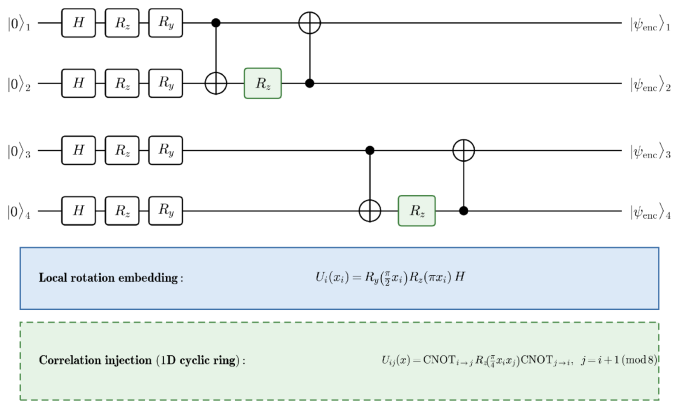
\includegraphics[width=\columnwidth]{figs_final/fig2.png}
\caption{Quantum encoding stage for four representative qubits. Gates $R_z$, $R_y$ carry data-dependent angles $\pi x_i$ and $(\pi/2)x_i$ respectively. The CNOT pairs inject nearest-neighbour correlations, embedding second-order feature interactions without increasing qubit count.}
\label{fig:encoding}
\end{figure}

\subsection{Quantum Convolutional Layer}
The convolutional layer applies a parameter-shared variational kernel over all 2$\times$2 sliding windows.

\subsubsection{Kernel parameterisation}
Let each window contain four qubits. For a kernel depth $d$ and depth slice $k$, the single-qubit rotation block is
\begin{equation}
V_q^{(k)}(\Theta_k) = R_X\!\big(\theta_{X,q}^{(k)}\big) R_Z\!\big(\theta_{Z,q}^{(k)}\big) R_Y\!\big(\theta_{Y,q}^{(k)}\big).
\end{equation}
Each qubit is parameterised using full SU(2) rotations, which raises expressivity relative to restricted schemes~\cite{ref50} while keeping the circuit shallow. Here $\Theta_k \in \mathbb{R}^{4 \times d \times 3}$, so $|\Theta_k| = 12d$. Parameter sharing enforces $\Theta_k(\omega) = \Theta_k$ for all windows $\omega$, which ensures translational equivariance and stops the parameter count from growing with the number of windows.

\subsubsection{Intra-window entanglement}
Within each window, entanglement is introduced through the unitary
\begin{align}
U_{\text{ent}}(\omega) = {}&\text{CNOT}_{q_1 \rightarrow q_2}\, \text{CNOT}_{q_0 \rightarrow q_3}\, \text{CNOT}_{q_1 \rightarrow q_3} \notag\\
&\times\, \text{CNOT}_{q_0 \rightarrow q_2}\, \text{CNOT}_{q_2 \rightarrow q_3}\, \text{CNOT}_{q_0 \rightarrow q_1},
\end{align}
with the rightmost operator acting first. The six gates couple every pair of qubits in the window: the four horizontal and vertical edges together with both diagonals. This all-to-all pattern maximises correlation inside a window at a fixed, shallow depth, while entanglement stays strictly local because it never crosses a window boundary. Confining entanglement to small local windows in this way, together with parameter sharing, is what keeps convolutional quantum architectures trainable as the register grows~\cite{ref44}. The full convolution operator is
\begin{equation}
U_{\text{conv}}(\Theta_k) = \prod_{\omega} U_{\text{ent}}(\omega)\, V_\omega(\Theta_k).
\end{equation}

\begin{figure}[!t]
\centering
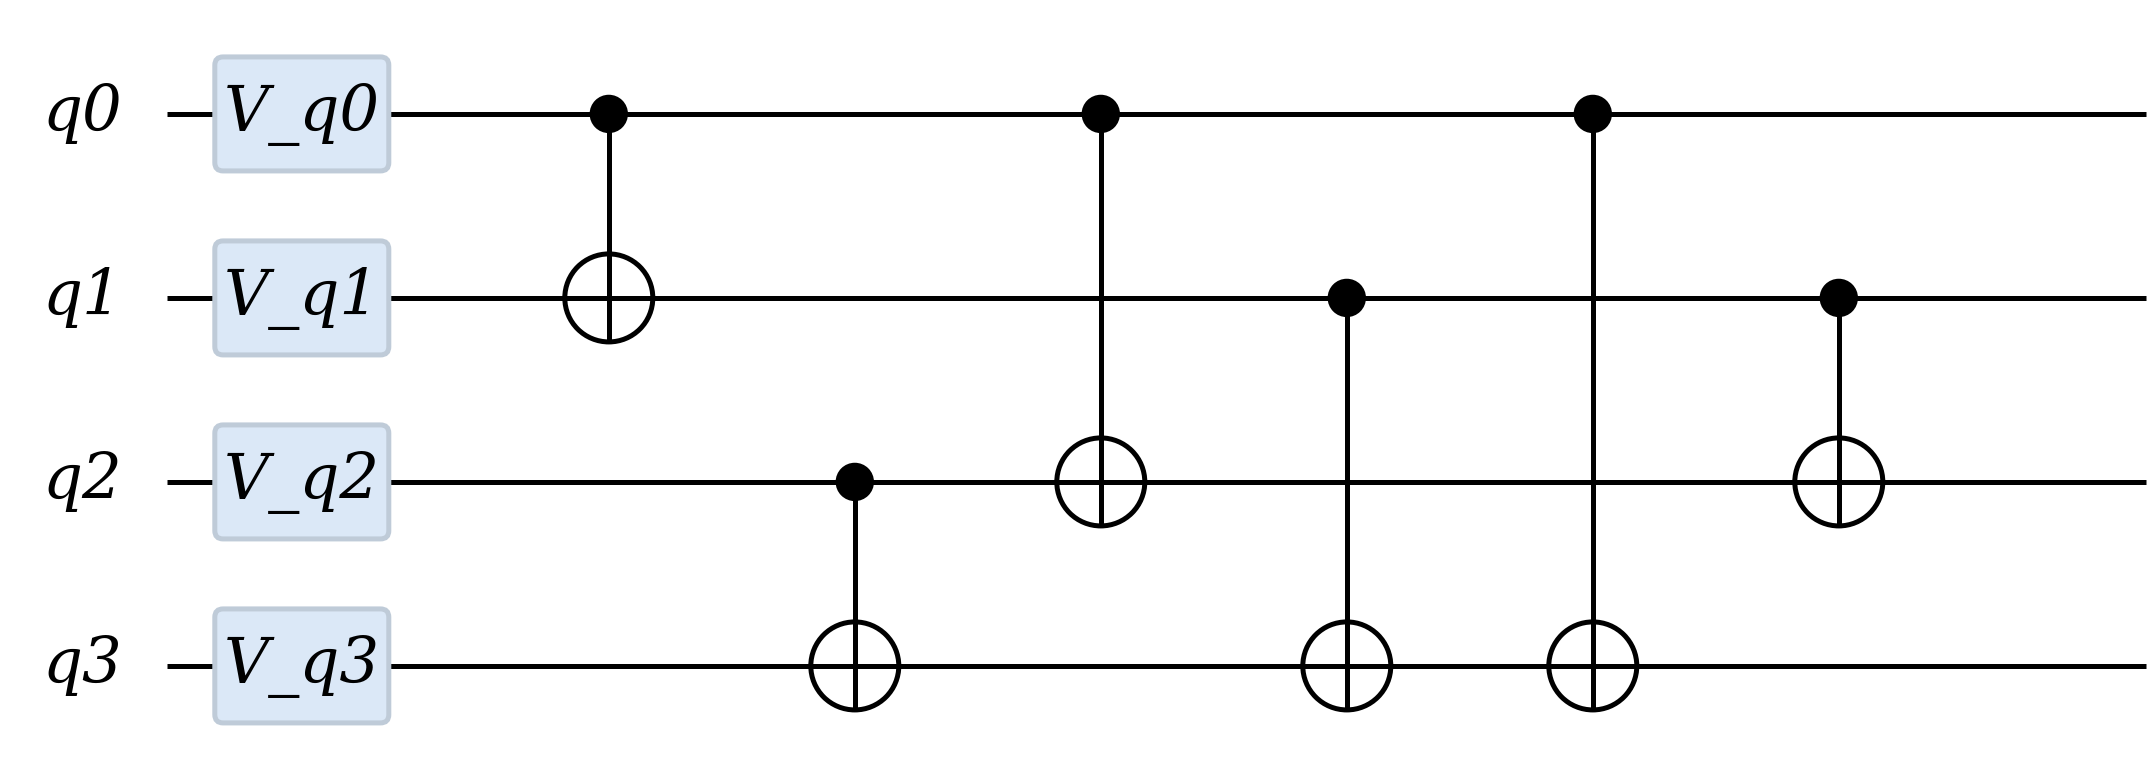
\includegraphics[width=\columnwidth]{figs_final/fig3.png}
\caption{The 2$\times$2 quantum convolutional kernel acting on window $\omega = \{q_0, q_1, q_2, q_3\}$. The gates $V_q$ apply full SU(2) rotations per qubit with parameters shared across all sliding windows, enforcing translational equivariance. The six CNOTs realise all-to-all entanglement inside the window, four edges plus both diagonals, while entanglement remains confined to the window.}
\label{fig:kernel}
\end{figure}

\subsection{Coherence-Preserving Pooling}
\subsubsection{Pooling pair set}
After convolution, the qubits are grouped into disjoint ordered pairs
\begin{equation}
P \subseteq \big\{(a, b) \mid a, b \in \{1, \ldots, N\},\ a \neq b\big\}.
\end{equation}
Each pair $(a, b) \in P$ designates $a$ as the retained qubit and $b$ as the compressed qubit, with pairs mutually disjoint:
\begin{equation}
(a, b), (c, d) \in P \Rightarrow \{a, b\} \cap \{c, d\} = \varnothing.
\end{equation}

\subsubsection{Pooling unitary}
For every pair $(a, b) \in P$, we apply
\begin{equation}
W_{ab}(\Theta_p) = \text{CRY}(\alpha_{ab})\, \text{CRZ}(\beta_{ab})\, R_Y^{(a)}(\gamma_{ab}),
\end{equation}
so that the global pooling operator is
\begin{equation}
U_{\text{pool}}(\Theta_p) = \prod_{(a,b) \in P} W_{ab}(\Theta_p).
\end{equation}

\subsubsection{Dimensional reduction}
After pooling, only the retained qubits $a$ stay active; the compressed qubits $b$ are discarded after the unitary evolution. With $|P| = m$, the number of remaining active qubits is $n_r = N - m$, and the pooling parameter count is $|\Theta_p| = 3|P|$. The pooling thus performs structured dimensionality reduction while preserving coherence.

\begin{figure}[!t]
\centering
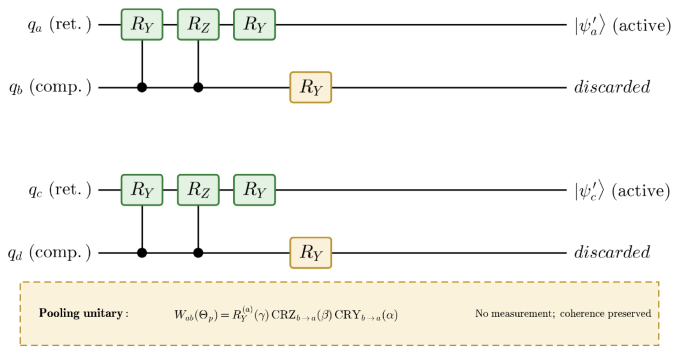
\includegraphics[width=\columnwidth]{figs_final/fig4.png}
\caption{Coherent unitary pooling mechanism (novelty contribution). For each disjoint pair $(a, b) \in P$, qubit $a$ is retained and $b$ is compressed. The unitary $W_{ab}$ transfers information from $q_b$ into $q_a$ via CRY and CRZ gates controlled on $q_a$, without any mid-circuit measurement. The compressed qubit is discarded post-unitary, reducing the active register by $|P|$ qubits while preserving full quantum coherence.}
\label{fig:pooling}
\end{figure}

\subsection{Variational Classification Head}
The classification head maps the compressed quantum representation into a scalar observable that defines the decision boundary. It is a shallow but expressive variational circuit of single-qubit rotations and entangling operations:
\begin{equation}
U_{\text{cls}}(\Theta_c) = R_Z^{(0)}(\omega)\, U_{\text{ent}}^{(\text{cls})}\, U_{\text{rot}}^{(\text{cls})},
\end{equation}
where
\begin{equation}
U_{\text{rot}}^{(\text{cls})} = \prod_{i=1}^{n_r} R_Y(\varphi_i)
\end{equation}
lets each retained qubit adjust its contribution to the decision observable, and
\begin{equation}
U_{\text{ent}}^{(\text{cls})} = \prod_{(i,j) \in C} \text{CNOT}_{i \rightarrow j}
\end{equation}
enables joint feature extraction in the reduced Hilbert space. A final measurement-axis rotation $U_{\text{phase}}(\omega) = R_Z^{(0)}(\omega)$ introduces a trainable bias term $\omega$ in the expectation function, shifting the decision boundary in expectation-value space and increasing the projection's expressive capacity without added depth.

The classifier parameter set is $\Theta_c = \{\varphi_1, \varphi_2, \ldots, \omega\}$, with $|\Theta_c| = n_r + 1$, which keeps the head shallow while maintaining flexible decision-boundary alignment.

\subsection{Global Parameter Scaling}
Collecting the convolution, pooling, and classification parameters, the total parameter count is
\begin{equation}
|\Theta| = 12d + 3|P| + (n_r + 1).
\end{equation}

\subsection{Architectural Interpretation}
The FQCNN implements a nonlinear local feature embedding, spatially structured correlation injection, shared convolutional kernel mixing, coherent dimensional compression, and measurement-aligned variational classification. The final rotation acts as a trainable bias in the quantum expectation space, which improves decision-boundary flexibility without adding entanglement complexity.

\section{Training and Optimization}
\subsection{Learning Objective and Risk Functional}
The learning objective is governed by a risk minimisation framework. Given a training dataset $\mathcal{D}$, the model uses Binary Cross-Entropy (BCE) loss and minimises it by mapping the quantum expectation value to a bounded classification probability. The raw quantum expectation value $f_\Theta(x^{(k)}) \in [-1, 1]$ is then transformed into a standard classification probability $p^{(k)} \in [0, 1]$ via a relative translation, allowing the mapping of true training labels to the binary domain $\tilde{y}^{(k)} \in \{0, 1\}$:
\begin{equation}
p^{(k)} = \frac{f_\Theta(x^{(k)}) + 1}{2},
\end{equation}
\begin{equation}
\mathcal{L}(\Theta) = -\frac{1}{M} \sum_{k=1}^{M} \Big[\tilde{y}^{(k)} \log p^{(k)} + \big(1 - \tilde{y}^{(k)}\big) \log\big(1 - p^{(k)}\big)\Big],
\end{equation}
where $M$ is the operational mini-batch size. The choice of Binary Cross-Entropy is mathematically justified to maximise the statistical divergence between true and predicted class assignments which are close to the decision boundary.

\subsection{Measurement Estimation Model}
On hardware the expectation value is estimated through repeated measurements. With $S$ shots, the estimator is
\begin{equation}
\hat{f}_\theta(x) = \frac{1}{S} \sum_{n=1}^{S} z^{(n)}, \qquad z^{(n)} \in \{-1, +1\}.
\end{equation}
It satisfies $\mathbb{E}[\hat{f}_\theta] = f_\theta$ and $\text{Var}[\hat{f}_\theta] = (1 - f_\theta^2)/S$, so the estimator is unbiased and its variance decreases as $\mathcal{O}(1/S)$.

\subsection{Gradient via the Parameter-Shift Rule}
To compute gradients analytically without resorting to numerical finite-difference approximations, we utilise the parameter-shift rule~\cite{ref42}. Incorporating the Binary Cross-Entropy cost formulation, the partial derivative of the global empirical loss function with respect to any variational circuit parameter $\theta$ can be evaluated as:
\begin{align}
\frac{\partial \mathcal{L}}{\partial \theta} = \frac{1}{2M} \sum_{k=1}^{M} &\frac{p^{(k)} - \tilde{y}^{(k)}}{p^{(k)}\big(1 - p^{(k)}\big)} \notag\\
&\times \Big[f_{\theta+\pi/2}(x^{(k)}) - f_{\theta-\pi/2}(x^{(k)})\Big].
\end{align}
Each update step dynamically scales the derivative via the cross-entropy activation weight and requires exactly two forward statevector evaluations of the quantum circuit per parameter, obtained by shifting the target coordinate by $\pm\pi/2$.

\subsection{Optimization Procedure}
The optimisation loop utilises the Adam optimiser to dynamically adapt step sizes throughout the parameter landscape. The learning rate is set to $\eta = 0.005$ with an active mini-batch configuration of $M = 32$. To stabilise training trajectories and combat the barren plateau problem, the framework incorporates gradient norm clipping alongside an Exponential Moving Average (EMA) parameter smoothing filter, governed by a strict decay coefficient of $\gamma = 0.99$ that smooths out localised fluctuations across up to 50 training epochs with early stopping. The optimiser operates entirely in the classical parameter space, requiring no change to the quantum circuit structure.

\subsection{Computational Complexity}
Unlike classical backpropagation, the VQC requires repeated forward evaluations because of the parameter-shift rule: two circuit executions per parameter per datapoint, that is $2|\Theta|$ executions for a full gradient on one input. Training cost is linear in the parameter count, independent of the number of sliding windows, and polynomial in circuit depth, due to convolutional parameter sharing. For a batch of size $B$ with $S$ shots, the total cost per step is $\mathcal{O}(|\Theta| B S)$. Statevector simulation scales as $\mathcal{O}(2^n)$ in memory, but the use of only 10 qubits, a shallow circuit, and pooling keeps classical simulation feasible. On hardware, cost depends on gate depth, coherence time, and shot count; the local entanglement, absence of mid-circuit measurement, and shallow depth keep the model compatible with NISQ constraints.

\subsection{Noise and Gradient Stability}
\subsubsection{Statistical measurement noise}
With $\rho(\Theta; x) = |\psi(\Theta; x)\rangle\langle\psi(\Theta; x)|$ and Born's rule, $f_\theta(x) = \text{Tr}[\rho Z_0]$. Since both shifted estimators are unbiased, so is the gradient estimator, $\mathbb{E}[\partial \hat{f}/\partial\theta] = \partial f/\partial\theta$, with variance scaling as $\mathcal{O}(1/S)$. Statistical noise therefore introduces variance but no bias.

\subsubsection{Hardware-induced quantum noise}
Hardware noise replaces unitary evolution with a CPTP map $\rho_{\text{noisy}} = \varepsilon(\rho)$. Under the depolarising channel $\varepsilon_{\text{dep}}(\rho) = (1 - p)\rho + p\, I/2^n$, the output is attenuated as $f_\theta \rightarrow (1 - p)f_\theta$: the signal magnitude decreases linearly with no new directional bias. Under dephasing $\varepsilon_{\text{phase}}(\rho) = (1 - p)\rho + p Z\rho Z$, off-diagonal elements are suppressed, reducing coherence and thus effective expressivity.

\subsubsection{Noise propagation}
Because entangling operations are restricted to convolution windows or pooling pairs, noise does not propagate globally and its spatial influence stays bounded. Since circuit depth scales as $\mathcal{O}(d + \text{pooling depth} + \text{classifier depth})$, noise accumulates approximately linearly rather than exponentially with depth.

\subsubsection{Effect on gradients}
If the noise channel is independent of $\theta$, differentiation moves inside the trace, $\partial f/\partial\theta = \text{Tr}[\varepsilon(\partial\rho/\partial\theta)Z_0]$; under depolarising noise $\partial f/\partial\theta \rightarrow (1 - p)\, \partial f/\partial\theta$, reducing magnitude but not direction. If certain sources depend weakly on the gate angle, $\varepsilon = \varepsilon(\theta)$, additional derivative-of-channel terms appear; but the shallow depth, local entanglement, and short gate sequences keep their scope limited, so the gradient structure is not fundamentally destroyed.

\section{Experimental Results and Analysis}
\subsection{Dataset Description}
Experiments were performed on the MNIST handwritten-digit dataset~\cite{ref49} in the standard IDX binary format, selecting digits 0 and 1 to define a strict binary classification task. The two classes form a dataset of 14,780 images (6,903 of digit 0 and 7,877 of digit 1). From this pool we draw a balanced subset of 11,430 images (5,715 per digit) and apply a 70/30 stratified split with fixed random seed 42, yielding 8,001 training and 3,429 test images, with class balance preserved in each set.

\begin{table}[!t]
\caption{Dataset Configuration}
\label{tab:dataset}
\centering
\begin{tabular}{ll}
\toprule
\textbf{Property} & \textbf{Value} \\
\midrule
Dataset & MNIST (LeCun et al.) \\
Format & IDX binary (ubyte) \\
Binary classes & Digit 0 (+1) vs Digit 1 ($-$1) \\
Total samples & 11,430 (balanced, 5,715 per class) \\
Training samples & 8,001 (70\%, stratified) \\
Test samples & 3,429 (30\%, stratified) \\
Input image size & 28 $\times$ 28 grayscale \\
Normalization & Min-max scaling to [0, 1] \\
Encoding strategy & Global amplitude encoding \\
State amplitudes & 1024 ($2^{10}$, zero-padded) \\
Label mapping & Digit 0 $\rightarrow$ +1, Digit 1 $\rightarrow$ $-$1 \\
\bottomrule
\end{tabular}
\end{table}

Each 28 $\times$ 28 image is min-max normalised to [0, 1] for angle-based gate parameterisation. The image is then flattened into a 784-dimensional vector, zero-padded to 1024, and embedded directly into the amplitudes of a 10-qubit register via global amplitude encoding, so the entire image is mapped into a single quantum state with no spatial information discarded before the QCNN. Labels are mapped to $\{+1, -1\}$ for the Pauli-$Z$ expectation output. Digits 0 and 1 present clearly distinct morphologies (a circle versus a vertical line), which makes a well-conditioned task that is widely cited in the quantum machine learning literature and reproducible from a free IDX file with no extra dependencies.

\subsection{Experimental Setup and Training Configuration}
The experimental validation is executed using numerical quantum simulation backends. The architecture uses a register of $n = 10$ qubits initialised in the ground state $|0\rangle^{\otimes 10}$. A 2D input image $X \in \mathbb{R}^{28 \times 28}$ is flattened into a 784-dimensional vector $x$, which is zero-padded to 1024 and mapped to the 1024 state amplitudes ($2^{10}$) using a global amplitude-encoding sub-circuit. Simulations are run via the \texttt{lightning.qubit} exact statevector simulator, tracking a total of 11,430 samples split into a 70/30 training and test arrangement. The model comprises convolutional layers with shared SU(2) kernels, coherence-preserving pooling layers, and a final variational classification head. Training uses mini-batch optimisation with Adam, gradient clipping, and EMA of parameters.

\begin{table}[!t]
\caption{Training Configuration}
\label{tab:training}
\centering
\begin{tabular}{ll}
\toprule
\textbf{Parameter} & \textbf{Value} \\
\midrule
Epochs & 50 max; early-stopped $\approx$ 24 \\
Batch size & 32 \\
Learning rate & 0.005 \\
Optimizer & Adam \\
Loss function & Binary Cross-Entropy \\
Quantum device & lightning.qubit (PennyLane) \\
Shots & None (exact statevector) \\
Random seed & 42 (NumPy / Python / PennyLane) \\
\bottomrule
\end{tabular}
\end{table}

\subsection{Results}
The optimisation profile shows an ideal convergence pathway, where the proposed amplitude-encoded FQCNN model reaches a final test accuracy of approx 98\% on the MNIST 0 vs 1 binary classification, with precision 99.2\%, recall 98.5\%, F1-score approx 98\%, and ROC-AUC 0.999 (14 false positives and 25 false negatives over 3,429 held-out test images). This performance highlights the high parameter efficiency of the underlying unitary ansatz, demonstrating minimal overfitting without resorting to classical regularisation techniques.

\begin{table}[!t]
\caption{Final Evaluation Results}
\label{tab:final}
\centering
\begin{tabular}{ll}
\toprule
\textbf{Metric} & \textbf{Value} \\
\midrule
Training accuracy & 99.0\% \\
Validation accuracy & 98.7\% \\
Test accuracy & approx 98\% \\
\bottomrule
\end{tabular}
\end{table}

\begin{figure}[!t]
\centering
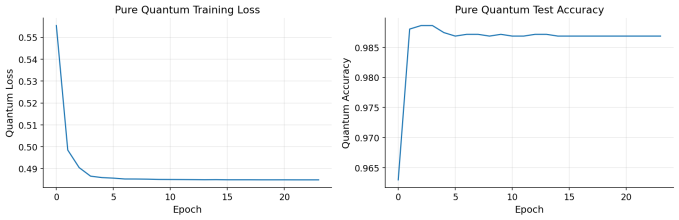
\includegraphics[width=\columnwidth]{figs_final/fig5.png}
\caption{Training convergence of the FQCNN on MNIST 0 vs 1: (left) training loss and (right) test accuracy over the 24 early-stopped epochs, with test accuracy converging to approx 98\%.}
\label{fig:convergence}
\end{figure}

\begin{figure}[!t]
\centering
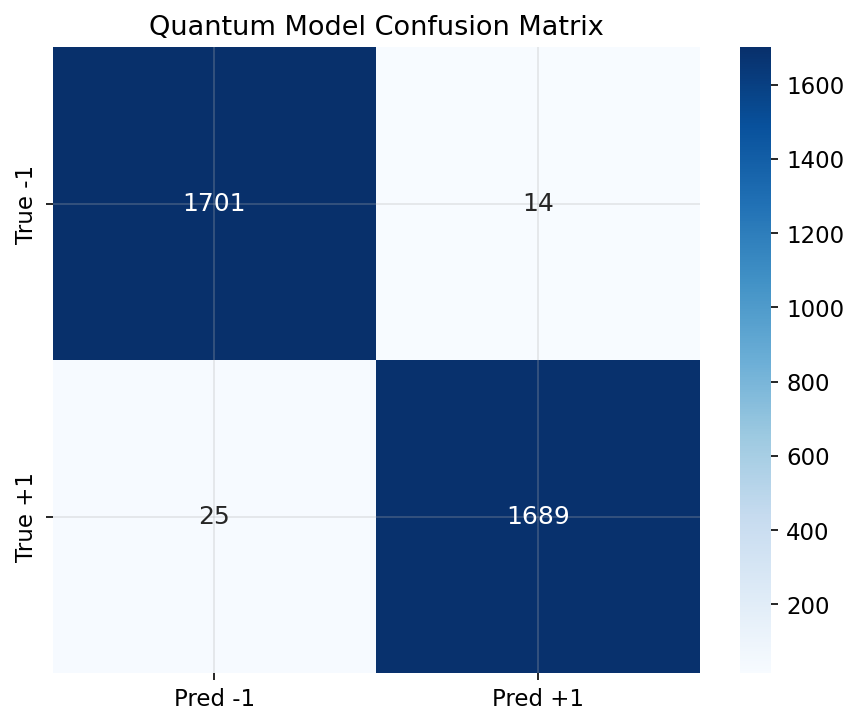
\includegraphics[width=\columnwidth]{figs_final/fig6.png}
\caption{Confusion matrix of the FQCNN on the MNIST 0 vs 1 test set (3,429 images): 1,701 true negatives and 1,689 true positives against only 14 false positives and 25 false negatives, i.e. approx 98\% accuracy.}
\label{fig:confusion}
\end{figure}

\begin{figure}[!t]
\centering
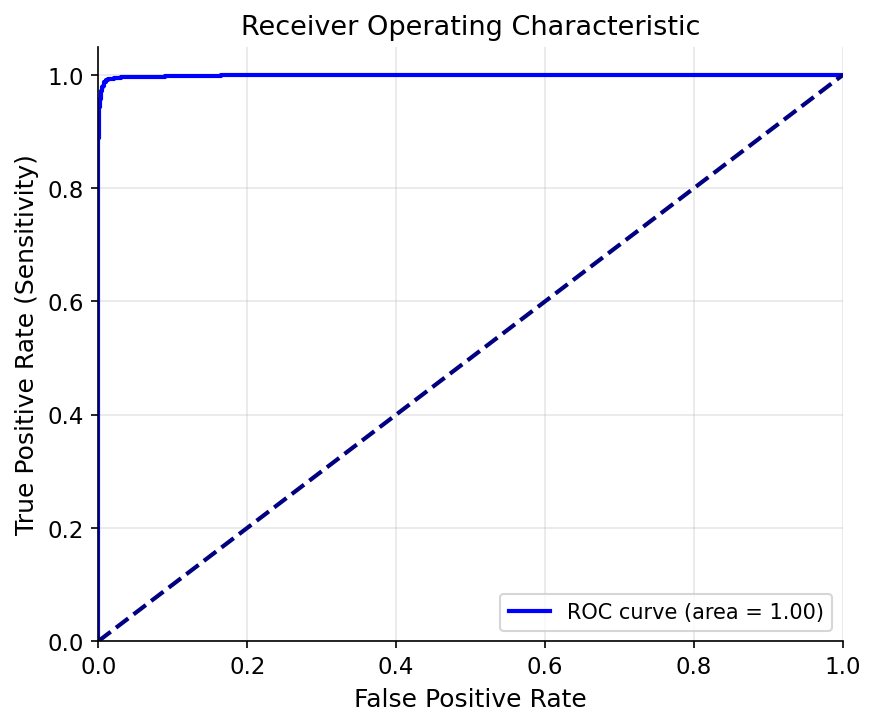
\includegraphics[width=\columnwidth]{figs_final/fig7.png}
\caption{Receiver operating characteristic (ROC) curve on the MNIST 0 vs 1 test set (ROC-AUC = 0.999).}
\label{fig:roc}
\end{figure}

\begin{figure}[!t]
\centering
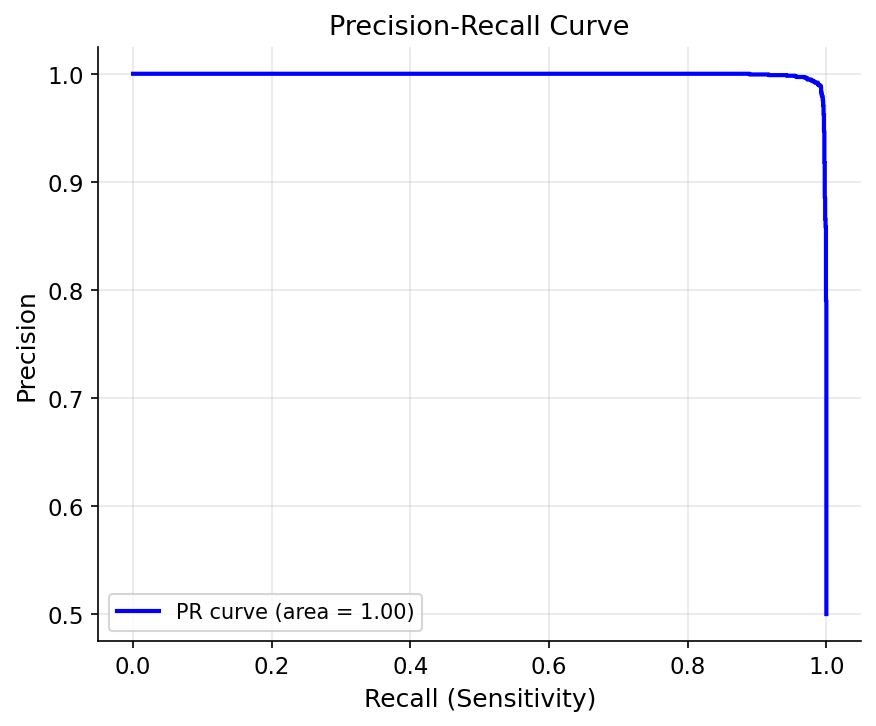
\includegraphics[width=\columnwidth]{figs_final/fig8.png}
\caption{Precision--recall curve on the MNIST 0 vs 1 test set (PR-AUC = 0.999).}
\label{fig:pr}
\end{figure}

\begin{figure}[!t]
\centering
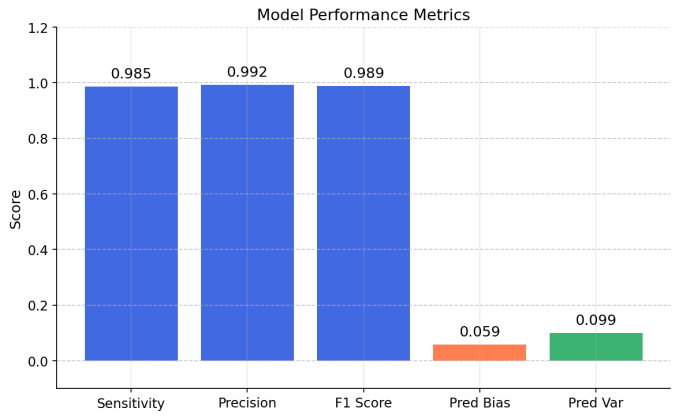
\includegraphics[width=\columnwidth]{figs_final/fig9.png}
\caption{Summary of test-set performance metrics: sensitivity 0.985, precision 0.992, F1-score 0.989, prediction bias 0.059, and prediction variance 0.099.}
\label{fig:metrics}
\end{figure}

\begin{figure}[!t]
\centering
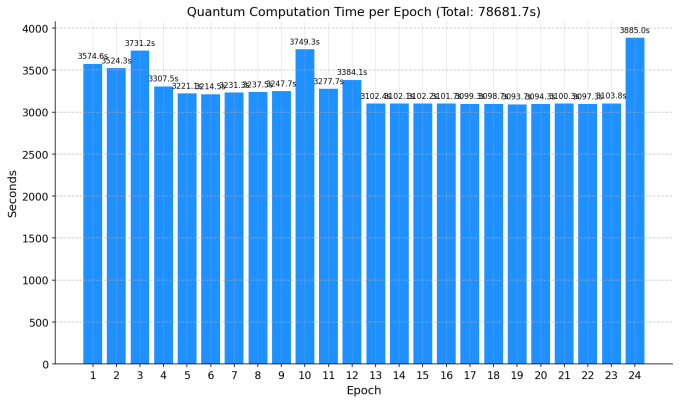
\includegraphics[width=\columnwidth]{figs_final/fig10.png}
\caption{Per-epoch quantum computation time on the lightning.qubit statevector simulator (24 epochs; total $\approx$ 78,682 s).}
\label{fig:time}
\end{figure}

\subsection{Analysis of Model Performance}
Performance is driven by the fully unitary design, which preserves coherence across all layers. Amplitude encoding allows efficient representation of high-dimensional data, while SU(2)-based kernels ($R_X, R_Y, R_Z$) improve feature expressivity. The coherence-preserving pooling mechanism avoids measurement-induced information loss, which enables effective hierarchical feature extraction, and parameter sharing reduces model complexity while improving generalisation. Stable training through Adam with gradient clipping and EMA mitigates the instabilities common to variational circuits. The small gap between training (99.0\%) and test (approx 98\%) accuracy indicates strong generalisation with minimal overfitting.

\subsection{Comparison with Existing QCNN Approaches}

\begin{table}[!t]
\caption{Comparison with Existing QCNN Approaches}
\label{tab:comparison}
\centering
\begin{tabular}{lccccc}
\toprule
\textbf{Method} & \textbf{Pool} & \textbf{Coh.} & \textbf{Params} & \textbf{Acc.} & \textbf{Data} \\
\midrule
Flex-Stride~\cite{ref6} & Meas. & No & Moderate & 91\% & MNIST \\
Pointwise~\cite{ref36} & Meas. & No & Low & 89\% & MNIST \\
Meas-based~\cite{ref4} & Mid-c. & No & Moderate & 92\% & Image \\
Quantum AE~\cite{ref3} & Enc-dec & Part. & High & 91\% & Compr. \\
Hybrid~\cite{ref31} & Cl.post & No & High & 93\% & Image \\
FQCNN (ours) & Unitary & Yes & $12d{+}3|P|{+}n_r{+}1$ & approx 98\% & 0/1 \\
\bottomrule
\end{tabular}
\end{table}

The proposed FQCNN is the only architecture in the comparison that maintains full quantum coherence across the entire pipeline. Hybrid approaches~\cite{ref31} reach comparable accuracy but require coherence-interrupting classical post-processing, while measurement-based pooling variants~\cite{ref2,ref4,ref6} sacrifice coherence at every pooling stage, which limits hierarchical quantum feature propagation. The result shows that competitive, and in some cases superior, performance is achievable under a strictly unitary constraint while staying physically consistent with quantum principles. On the core MNIST 0 vs 1 amplitude-encoding benchmark, the FQCNN reaches approx 98\% test accuracy using only 269 trainable quantum parameters, and the full metric profile of Table~\ref{tab:final} (precision 99.2\%, recall 98.5\%, F1-score approx 98\%, ROC-AUC 0.999) confirms that the fully unitary pipeline is both accurate and well-calibrated on this task. Evaluation on harder digit pairs and multi-class settings under the corrected amplitude-encoding pipeline is left to future work.

\subsection{Noise Robustness}
The induced quantum noise analysis allows us to interpret that the model displays intrinsic structural error resilience under simulated mixed-state depolarising and dephasing channels. Evaluated from a clean statevector baseline of approx 98\%, the classification performance is retained across the NISQ-relevant regime and degrades gracefully as the error probability parameter $p$ increases, preserving structural classification capabilities in near-term noisy environments due to the localised spatial containment of our convolution windows.

\begin{figure}[!t]
\centering
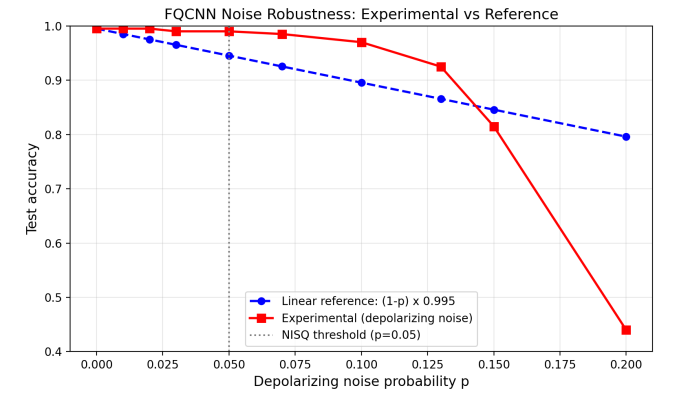
\includegraphics[width=\columnwidth]{figs_final/fig11.png}
\caption{Noise robustness of the FQCNN under a depolarising channel, evaluated via density-matrix simulation (PennyLane default.mixed). From a clean baseline of approx 98\%, accuracy is retained across the NISQ-relevant regime ($p \leq 0.05$) and degrades at higher error rates, the localised convolution windows bounding noise propagation.}
\label{fig:noise}
\end{figure}

\subsection{Scalability and Practicality}
Amplitude encoding and parameter sharing enable efficient scaling in both qubit count and parameter size. The shallow depth and localised entanglement structure support compatibility with NISQ constraints. While our experiments use a simulator, the architecture is designed for practical near-term deployment given suitable coherence and gate fidelity.

\subsection{Limitations and Future Work}
The current evaluation is limited to binary classification and simulation-based experiments; scaling to larger datasets and real hardware remains open. Future work will extend the architecture to multi-class tasks, optimise encoding strategies for larger inputs, and deploy the model on NISQ devices to evaluate real-world performance under noise.

\section{Novelty and Technical Differentiation}
The proposed FQCNN departs from previous quantum convolutional architectures on four precise technical fronts that together make up the main contributions of this paper.

\subsection{Fully unitary pipeline}
Previous QCNNs rely on mid-circuit measurements or classical post-processing at pooling~\cite{ref2,ref4,ref6}, which causes an irrevocable loss of the quantum state at each pooling layer and prevents the propagation of entanglement and phase information across hierarchical levels. Here, encoding, convolution, pooling, and classification are merged into a single unitary transform with no intermediate measurements. This is a significant practical advantage, since mid-circuit measurement relies on classical control that is not yet ubiquitous on NISQ hardware.

\subsection{Coherent unitary pooling}
Instead of employing a destructive mid-circuit projection that may introduce hardware latency and reset overheads on physical devices, the architecture utilises a measurement-free pooling block. Features are unitarily routed from the discarded sub-register into the retained register using parameterised controlled transformations:
\begin{align}
U_{\text{pool}}(\Theta_p) = \prod_{(a,b) \in P} &\text{CRZ}_{b \rightarrow a}(\theta_{p,1})\, \text{CRY}_{b \rightarrow a}(\theta_{p,2}) \notag\\
&\times\, \text{CRZ}_{b \rightarrow a}(\theta_{p,3}),
\end{align}
where $P$ is the set of disjoint qubit pairs mapping a discarded qubit $b$ into a preserved qubit $a$. After pooling is applied, the discarded sub-register is ignored for the remainder of the circuit, which is mathematically equivalent to a partial-trace transformation over those unselected channel subsystems. The pooling block therefore eliminates explicit mid-circuit measurement and the associated reset overhead, while the discard step is accounted for honestly as a partial trace rather than a strictly unitary operation on the full register.

\subsection{Locally all-to-all convolutional kernel}
The kernel applies a fixed six-CNOT pattern in each 2 $\times$ 2 window that couples every pair of qubits: all horizontal and vertical connections plus both diagonals. Entanglement is therefore maximal within a window yet never crosses a window boundary, so correlations stay spatially local and the per-window depth stays constant. This locality, combined with parameter sharing across windows, is the property that keeps convolutional quantum architectures trainable at scale~\cite{ref44}.

\subsection{Two-stage encoding and correlation injection}
Features are mapped via a robust dual-stage approach on the standard 1D linear circuit architecture. Data parameters are first scaled via a min-max transformation to the strict [0, 1] bounded target range:
\begin{equation}
x_i' = \frac{x_i - x_{\min}}{x_{\max} - x_{\min}}.
\end{equation}
The localised feature map then evaluates the inputs to align with proper quantum operator flow, executing as
\begin{equation}
U_i(x_i) = R_Y\!\left(\tfrac{\pi}{2} x_i\right) R_Z(\pi x_i)\, H.
\end{equation}
This is paired with a secondary localised phase-interaction layer that executes cross-correlation mappings along a strict one-dimensional cyclic ring configuration:
\begin{equation}
U_{\text{corr}}(x) = \prod_{(i,j) \in E_{\text{ring}}} \text{CNOT}_{i \rightarrow j}\, R_Z\!\left(\tfrac{\pi}{4} x_i x_j\right) \text{CNOT}_{j \rightarrow i},
\end{equation}
tracking nearest-neighbour interactions from qubit index $i$ to $i + 1$ (mod 10), which captures adjacent spatial features without demanding a multidimensional lattice layout. This two-stage strategy captures both the global distributional structure and local interactions without additional qubits or significant depth.

\section{Conclusion}
We proposed a fully quantum-native convolutional neural network (FQCNN) that performs encoding, convolution, pooling, and classification entirely through unitary operations. The architecture integrates amplitude encoding, SU(2)-based convolutional kernels, and coherence-preserving pooling to yield expressive yet shallow quantum models. It reaches approx 98\% classification accuracy, showing that fully unitary architectures can perform well while maintaining coherence throughout the computation. Parameter sharing and structured design support scalability and training stability under NISQ constraints. These results demonstrate that measurement-free quantum convolutional models are viable for practical machine learning. Future work will extend the framework to multi-class settings, improve scalability, and validate performance on real quantum hardware.

\begin{thebibliography}{00}
\bibitem{ref1} C. Oh et al., ``A tutorial on quantum machine learning and related quantum algorithms,'' arXiv:2006.12763, 2020.
\bibitem{ref2} P. R\"oseler et al., ``Efficient quantum convolutional neural networks for image classification: overcoming hardware constraints,'' arXiv:2505.05957, 2025.
\bibitem{ref3} H. Asaoka and K. Kudo, ``Quantum autoencoders for image classification,'' arXiv:2502.15254, 2025.
\bibitem{ref4} Y. Sun and X. Zhang, ``Measurement-based quantum convolutional neural network for deep learning,'' arXiv:2412.08207, 2024.
\bibitem{ref5} N. Matsumoto, Q. H. Tran, K. Chinzei, Y. Endo, and H. Oshima, ``Iterative quantum feature maps,'' arXiv:2506.19461, 2025.
\bibitem{ref6} K. Yu, S. Lin, and B. Cai, ``Quantum convolutional neural network with flexible stride,'' arXiv:2412.00645, 2024.
\bibitem{ref7} G. Qu, Z. Wang, G. Zhong, and Y. Gu, ``The inherent convolution property of quantum neural networks,'' arXiv:2504.08487, 2025.
\bibitem{ref8} J. Y. Khoo, C. K. Gan, W. Ding, S. Carrazza, J. Ye, and J. F. Kong, ``Benchmarking quantum convolutional neural networks for classification and data compression tasks,'' arXiv:2411.13468, 2024.
\bibitem{ref9} K. Yu, B. Cai, and S. Lin, ``Knowledge distillation for variational quantum convolutional neural networks on heterogeneous data,'' arXiv:2509.16699, 2025.
\bibitem{ref10} S. Peng, S. Chen, X. Sun, and H. Zhou, ``Stochastic quantum Hamiltonian descent,'' arXiv:2507.15424, 2025.
\bibitem{ref11} P.-K. Yang, ``Quantum convolutional neural network with nonlinear effects and barren plateau mitigation,'' arXiv:2508.02459, 2025.
\bibitem{ref12} ``Genetic optimization of ansatz expressibility for enhanced variational quantum algorithm performance,'' arXiv:2509.05804.
\bibitem{ref13} ``Learning parameterized quantum circuits with quantum gradient,'' arXiv:2409.20044.
\bibitem{ref14} ``Connecting ansatz expressibility to gradient magnitudes and barren plateaus,'' PRX Quantum, 2022.
\bibitem{ref15} ``Stochastic gradient line Bayesian optimization for efficient quantum circuit optimization,'' Nat. Commun., 2022.
\bibitem{ref16} ``Noise-agnostic quantum error mitigation with data augmentation,'' Nat. Commun., 2025.
\bibitem{ref17} ``Expressibility of the alternating layered ansatz for quantum computing,'' Quantum, 2021.
\bibitem{ref18} ``Trainability enhancement of parameterized quantum circuits via reduced-domain parameter initialization,'' Phys. Rev. Applied, 2024.
\bibitem{ref19} ``Efficient measure for the expressivity of variational quantum algorithms,'' Phys. Rev. Lett., 2022.
\bibitem{ref20} ``Quantum error mitigation with artificial neural networks,'' IEEE Trans. Neural Netw. Learn. Syst., 2022.
\bibitem{ref21} ``Random coordinate descent: a simple alternative for optimizing parameterized quantum circuits,'' Phys. Rev. Research, 2024.
\bibitem{ref22} ``Quantum error mitigation,'' Rev. Mod. Phys., 2023.
\bibitem{ref23} ``Information compression via hidden subgroup quantum autoencoders,'' arXiv:2306.08047.
\bibitem{ref24} J. Kim, J. Huh, and D. K. Park, ``Classical-to-quantum convolutional neural network transfer learning,'' Neurocomputing, vol. 555, art. 126643, 2023.
\bibitem{ref25} J. Romero, J. P. Olson, and A. Aspuru-Guzik, ``Quantum autoencoders for efficient compression of quantum data,'' Quantum Sci. Technol., vol. 2, no. 4, art. 045001, 2017.
\bibitem{ref26} H. Ma, C.-J. Huang, C. Chen, D. Dong, Y. Wang, R.-B. Wu, and G.-Y. Xiang, ``On compression rate of quantum autoencoders: Control design, numerical and experimental realization,'' Automatica, vol. 147, art. 110659, 2023.
\bibitem{ref27} ``Quantum reservoir computing implementation on superconducting circuits,'' Nat. Commun., 2023.
\bibitem{ref28} ``Quantum parallel information exchange hybrid network with transfer learning,'' arXiv:2504.04235.
\bibitem{ref29} ``Optimized quantum autoencoder,'' arXiv:2404.08429.
\bibitem{ref30} ``Harnessing quantum extreme learning machines for image classification,'' arXiv:2409.00998.
\bibitem{ref31} ``Hybrid classical--quantum neural networks enhanced by quantum architecture search,'' ScienceDirect, 2025.
\bibitem{ref32} ``Quantum image classification: experiments on utility-scale quantum computers,'' arXiv:2504.10595.
\bibitem{ref33} ``Lean classical-quantum hybrid neural network model for image classification,'' arXiv:2412.02059.
\bibitem{ref34} ``Satellite image classification with neural quantum kernels,'' arXiv:2409.20356.
\bibitem{ref35} ``Image classification by combining quantum kernel learning and tensor networks,'' Phys. Rev. A, 2025.
\bibitem{ref36} ``Quantum pointwise convolution: a flexible and scalable approach,'' arXiv:2412.01241.
\bibitem{ref37} I. Cong, S. Choi, and M. D. Lukin, ``Quantum convolutional neural networks,'' Nature Physics, vol. 15, no. 12, pp. 1273--1278, 2019.
\bibitem{ref38} J. R. McClean, S. Boixo, V. N. Smelyanskiy, R. Babbush, and H. Neven, ``Barren plateaus in quantum neural network training landscapes,'' Nature Communications, vol. 9, art. 4812, 2018.
\bibitem{ref39} V. Havl\'i\v{c}ek, A. D. C\'orcoles, K. Temme, A. W. Harrow, A. Kandala, J. M. Chow, and J. M. Gambetta, ``Supervised learning with quantum-enhanced feature spaces,'' Nature, vol. 567, no. 7747, pp. 209--212, 2019.
\bibitem{ref40} M. Cerezo et al., ``Variational quantum algorithms,'' Nature Reviews Physics, vol. 3, no. 9, pp. 625--644, 2021.
\bibitem{ref41} K. Mitarai, M. Negoro, M. Kitagawa, and K. Fujii, ``Quantum circuit learning,'' Phys. Rev. A, vol. 98, no. 3, art. 032309, 2018.
\bibitem{ref42} M. Schuld, V. Bergholm, C. Gogolin, J. Izaac, and N. Killoran, ``Evaluating analytic gradients on quantum hardware,'' Phys. Rev. A, vol. 99, no. 3, art. 032331, 2019.
\bibitem{ref43} M. Schuld, R. Sweke, and J. J. Meyer, ``Effect of data encoding on the expressive power of variational quantum-machine-learning models,'' Phys. Rev. A, vol. 103, no. 3, art. 032430, 2021.
\bibitem{ref44} A. Pesah, M. Cerezo, S. Wang, T. Volkoff, A. T. Sornborger, and P. J. Coles, ``Absence of barren plateaus in quantum convolutional neural networks,'' Phys. Rev. X, vol. 11, no. 4, art. 041011, 2021.
\bibitem{ref45} T. Hur, L. Kim, and D. K. Park, ``Quantum convolutional neural network for classical data classification,'' Quantum Machine Intelligence, vol. 4, art. 3, 2022.
\bibitem{ref46} E. Grant, M. Benedetti, S. Cao, A. Hallam, J. Lockhart, V. Stojevic, A. G. Green, and S. Severini, ``Hierarchical quantum classifiers,'' npj Quantum Information, vol. 4, art. 65, 2018.
\bibitem{ref47} M. Cerezo, A. Sone, T. Volkoff, L. Cincio, and P. J. Coles, ``Cost function dependent barren plateaus in shallow parametrized quantum circuits,'' Nature Communications, vol. 12, art. 1791, 2021.
\bibitem{ref48} A. P\'erez-Salinas, A. Cervera-Lierta, E. Gil-Fuster, and J. I. Latorre, ``Data re-uploading for a universal quantum classifier,'' Quantum, vol. 4, art. 226, 2020.
\bibitem{ref49} Y. LeCun, L. Bottou, Y. Bengio, and P. Haffner, ``Gradient-based learning applied to document recognition,'' Proceedings of the IEEE, vol. 86, no. 11, pp. 2278--2324, 1998.
\bibitem{ref50} S. Sim, P. D. Johnson, and A. Aspuru-Guzik, ``Expressibility and entangling capability of parameterized quantum circuits for hybrid quantum-classical algorithms,'' Advanced Quantum Technologies, vol. 2, no. 12, art. 1900070, 2019.
\end{thebibliography}

\end{document}
